\documentclass[xcolor={dvipsnames}]{beamer}
%\usepackage[utf8]{inputenc}
\usetheme{Madrid}
%\usetheme{Malmoe}
\usecolortheme{beaver}
%\usecolortheme{rose}

%-------------------------------------------------------------------------------
%          -Packages nécessaires pour écrire en Français et en UTF8-
%-------------------------------------------------------------------------------
\usepackage[utf8]{inputenc}
\usepackage[frenchb]{babel}
\usepackage[T1]{fontenc}
\usepackage{lmodern}
\usepackage{textcomp}

%-------------------------------------------------------------------------------

%-------------------------------------------------------------------------------
%                          -Outils de mise en forme-
%-------------------------------------------------------------------------------
\usepackage{hyperref}
\hypersetup{pdfstartview=XYZ}
\usepackage{enumerate}
\usepackage{graphicx}
%\usepackage{multicol}
%\usepackage{tabularx}

%\usepackage{anysize} %%pour pouvoir mettre les marges qu'on veut
%\marginsize{2.5cm}{2.5cm}{2.5cm}{2.5cm}

\usepackage{indentfirst} %%pour que les premier paragraphes soient aussi indentés
\usepackage{verbatim}
%\usepackage[table]{xcolor}  
%\usepackage{multirow}
\usepackage{ulem}
%-------------------------------------------------------------------------------


%-------------------------------------------------------------------------------
%                  -Nécessaires pour écrire des mathématiques-
%-------------------------------------------------------------------------------
\usepackage{amsfonts}
\usepackage{amssymb}
\usepackage{amsmath}
\usepackage{amsthm}
\usepackage{tikz}
\usepackage{xlop}
\usepackage[output-decimal-marker={,}]{siunitx}
%-------------------------------------------------------------------------------


%-------------------------------------------------------------------------------
%                    - Mise en forme 
%-------------------------------------------------------------------------------

\newcommand{\bu}[1]{\underline{\textbf{#1}}}


\usepackage{ifthen}


\newcommand{\ifTrue}[2]{\ifthenelse{\equal{#1}{true}}{#2}{$\qquad \qquad$}}

\newcommand{\kword}[1]{\textcolor{red}{\underline{#1}}}


%-------------------------------------------------------------------------------



%-------------------------------------------------------------------------------
%                    - Racourcis d'écriture -
%-------------------------------------------------------------------------------

% Angles orientés (couples de vecteurs)
\newcommand{\aopp}[2]{(\vec{#1}, \vec{#2})} %Les deuc vecteurs sont positifs
\newcommand{\aopn}[2]{(\vec{#1}, -\vec{#2})} %Le second vecteur est négatif
\newcommand{\aonp}[2]{(-\vec{#1}, \vec{#2})} %Le premier vecteur est négatif
\newcommand{\aonn}[2]{(-\vec{#1}, -\vec{#2})} %Les deux vecteurs sont négatifs

%Ensembles mathématiques
\newcommand{\naturels}{\mathbb{N}} %Nombres naturels
\newcommand{\relatifs}{\mathbb{Z}} %Nombres relatifs
\newcommand{\rationnels}{\mathbb{Q}} %Nombres rationnels
\newcommand{\reels}{\mathbb{R}} %Nombres réels
\newcommand{\complexes}{\mathbb{C}} %Nombres complexes


%Intégration des parenthèses aux cosinus
\newcommand{\cosP}[1]{\cos\left(#1\right)}
\newcommand{\sinP}[1]{\sin\left(#1\right)}

%Fractions
\newcommand{\myfrac}[2]{{\LARGE $\frac{#1}{#2}$}}

%Vocabulaire courrant
\newcommand{\cad}{c'est-à-dire}

%Droites
\newcommand{\dte}[1]{droite $(#1)$}
\newcommand{\fig}[1]{figure $#1$}
\newcommand{\sym}{symétrique}
\newcommand{\syms}{symétriques}
\newcommand{\asym}{axe de symétrie}
\newcommand{\asyms}{axes de symétrie}
\newcommand{\seg}[1]{$[#1]$}
\newcommand{\monAngle}[1]{$\widehat{#1}$}
\newcommand{\bissec}{bissectrice}
\newcommand{\mediat}{médiatrice}
\newcommand{\ddte}[1]{$[#1)$}

%Figures
\newcommand{\para}{parallélogramme}
\newcommand{\paras}{parallélogrammes}
\newcommand{\myquad}{quadrilatère}
\newcommand{\myquads}{quadrilatères}
\newcommand{\co}{côtés opposés}
\newcommand{\diag}{diagonale}
\newcommand{\diags}{diagonales}
\newcommand{\supp}{supplémentaires}
\newcommand{\car}{carré}
\newcommand{\cars}{carrés}
\newcommand{\rect}{rectangle}
\newcommand{\rects}{rectangles}
\newcommand{\los}{losange}
\newcommand{\loss}{losanges}


%----------------------------------------------------


\usepackage{../../../../pas-math}
\usepackage{../../../../moncours_beamer}

\usepackage{amssymb,amsmath}


\newcommand{\myitem}{\item[\textbullet]}

\graphicspath{{../img/}}

\title{Séquence 5 : Nombres relatifs}
%\author{O. FINOT}\institute{Collège S$^t$ Bernard}
\date{}

%
\AtBeginSection[]
{
	\begin{frame}
		\frametitle{}
		\tableofcontents[currentsection, hideallsubsections]
	\end{frame} 

}
%
%
%\AtBeginSubsection[]
%{
%	\begin{frame}
%		\frametitle{Sommaire}
%		\tableofcontents[currentsection, currentsubsection]
%	\end{frame} 
%}

\begin{document}



\begin{frame}
  \titlepage 
\end{frame}


	

\begin{frame}
	\begin{block}{Objectifs}
		\begin{itemize}
			
		\item Savoir ce qu’est un nombre relatif et connaître le vocabulaire associé.
		\item Savoir comparer des nombres relatifs.
		\item Savoir additionner et soustraire des nombres relatifs.
		\item Savoir sur repérer sur un axe ou dans le le plan.
			
			\end{itemize}
	\end{block}
\end{frame}

\begin{frame}
	\begin{block}{Compétences travaillées}
		\begin{itemize}
			\item \kword{Représenter (Re2)} :  produire et utiliser plusieurs représentations d’un nombre;
			\item \kword{Calculer (Ca1)} :  calculer avec des nombres rationnels, de manière exacte ou approchée en combinant astucieusement le calcul mental, le calcul posé et le calcul instrumenté ;
			\item \kword{Raisonner (Ra1)} :  résoudre des problèmes impliquant des grandeurs variées : mobiliser les connaissances nécessaires, analyser et exploiter ses erreurs, mettre à l’essai plusieurs solutions.		
		\end{itemize}
	\end{block}
\end{frame}



\section{Définitions}




\begin{frame}
	\begin{mydefs}
		\begin{itemize}
			\item Un nombre supérieur à 0 est un \kword{nombre positif},\pause un nombre inférieur à 0 est un \kword{nombre négatif}.
			
			\begin{center}
				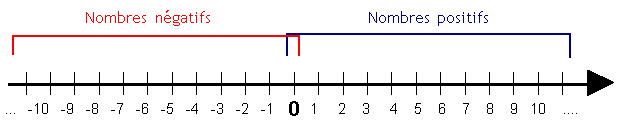
\includegraphics[scale=0.5]{relatifs}\pause
			\end{center}
			
			\item Les nombres positifs et négatifs forment l'ensembles des \kword{nombres relatifs}.\pause
			
			\item Un nombre relatif est composé d'\kword{un signe} (+ ou -) et d'une \kword{distance à zéro}.\pause
			
			\item Deux \kword{nombres opposés} ont la \kword{même distance à zéro} et des \kword{signes différents}. 
			
			
		\end{itemize}
	\end{mydefs}
	
\end{frame}


\begin{frame}
	\begin{myexs}
		\begin{itemize}
			\item $+7$ est un nombre \pause positif, sa distance à zéro est \pause $7$; 
			\begin{center}
				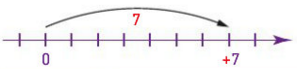
\includegraphics[scale=0.6]{ex1}\pause
			\end{center}
			\item $\num{-4}$ est un nombre \pause négatif, sa distance à zéro est \pause $\num{4}$;
			\begin{center}
				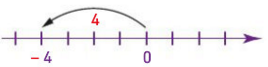
\includegraphics[scale=0.6]{ex2}\pause
			\end{center}
			
			\item $0$ est \pause à la fois un nombre positif et négatif.%, sa distance à zéro est 0.
			\item $-10$ et $+10$ sont \pause opposés.
			\begin{center}
				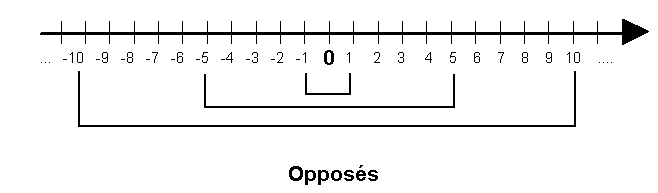
\includegraphics[scale=0.5]{opposes}
			\end{center}
		\end{itemize}
	\end{myexs}
\end{frame}

\section{Des nombres pour se repérer et à comparer}

%\subsection{Repérage}

\begin{mydef}
	Sur une droite graduée, chaque point est repéré par un nombre relatif, son %\kw{abscisse}.
\end{mydef}


\begin{myex}
	\begin{center}
		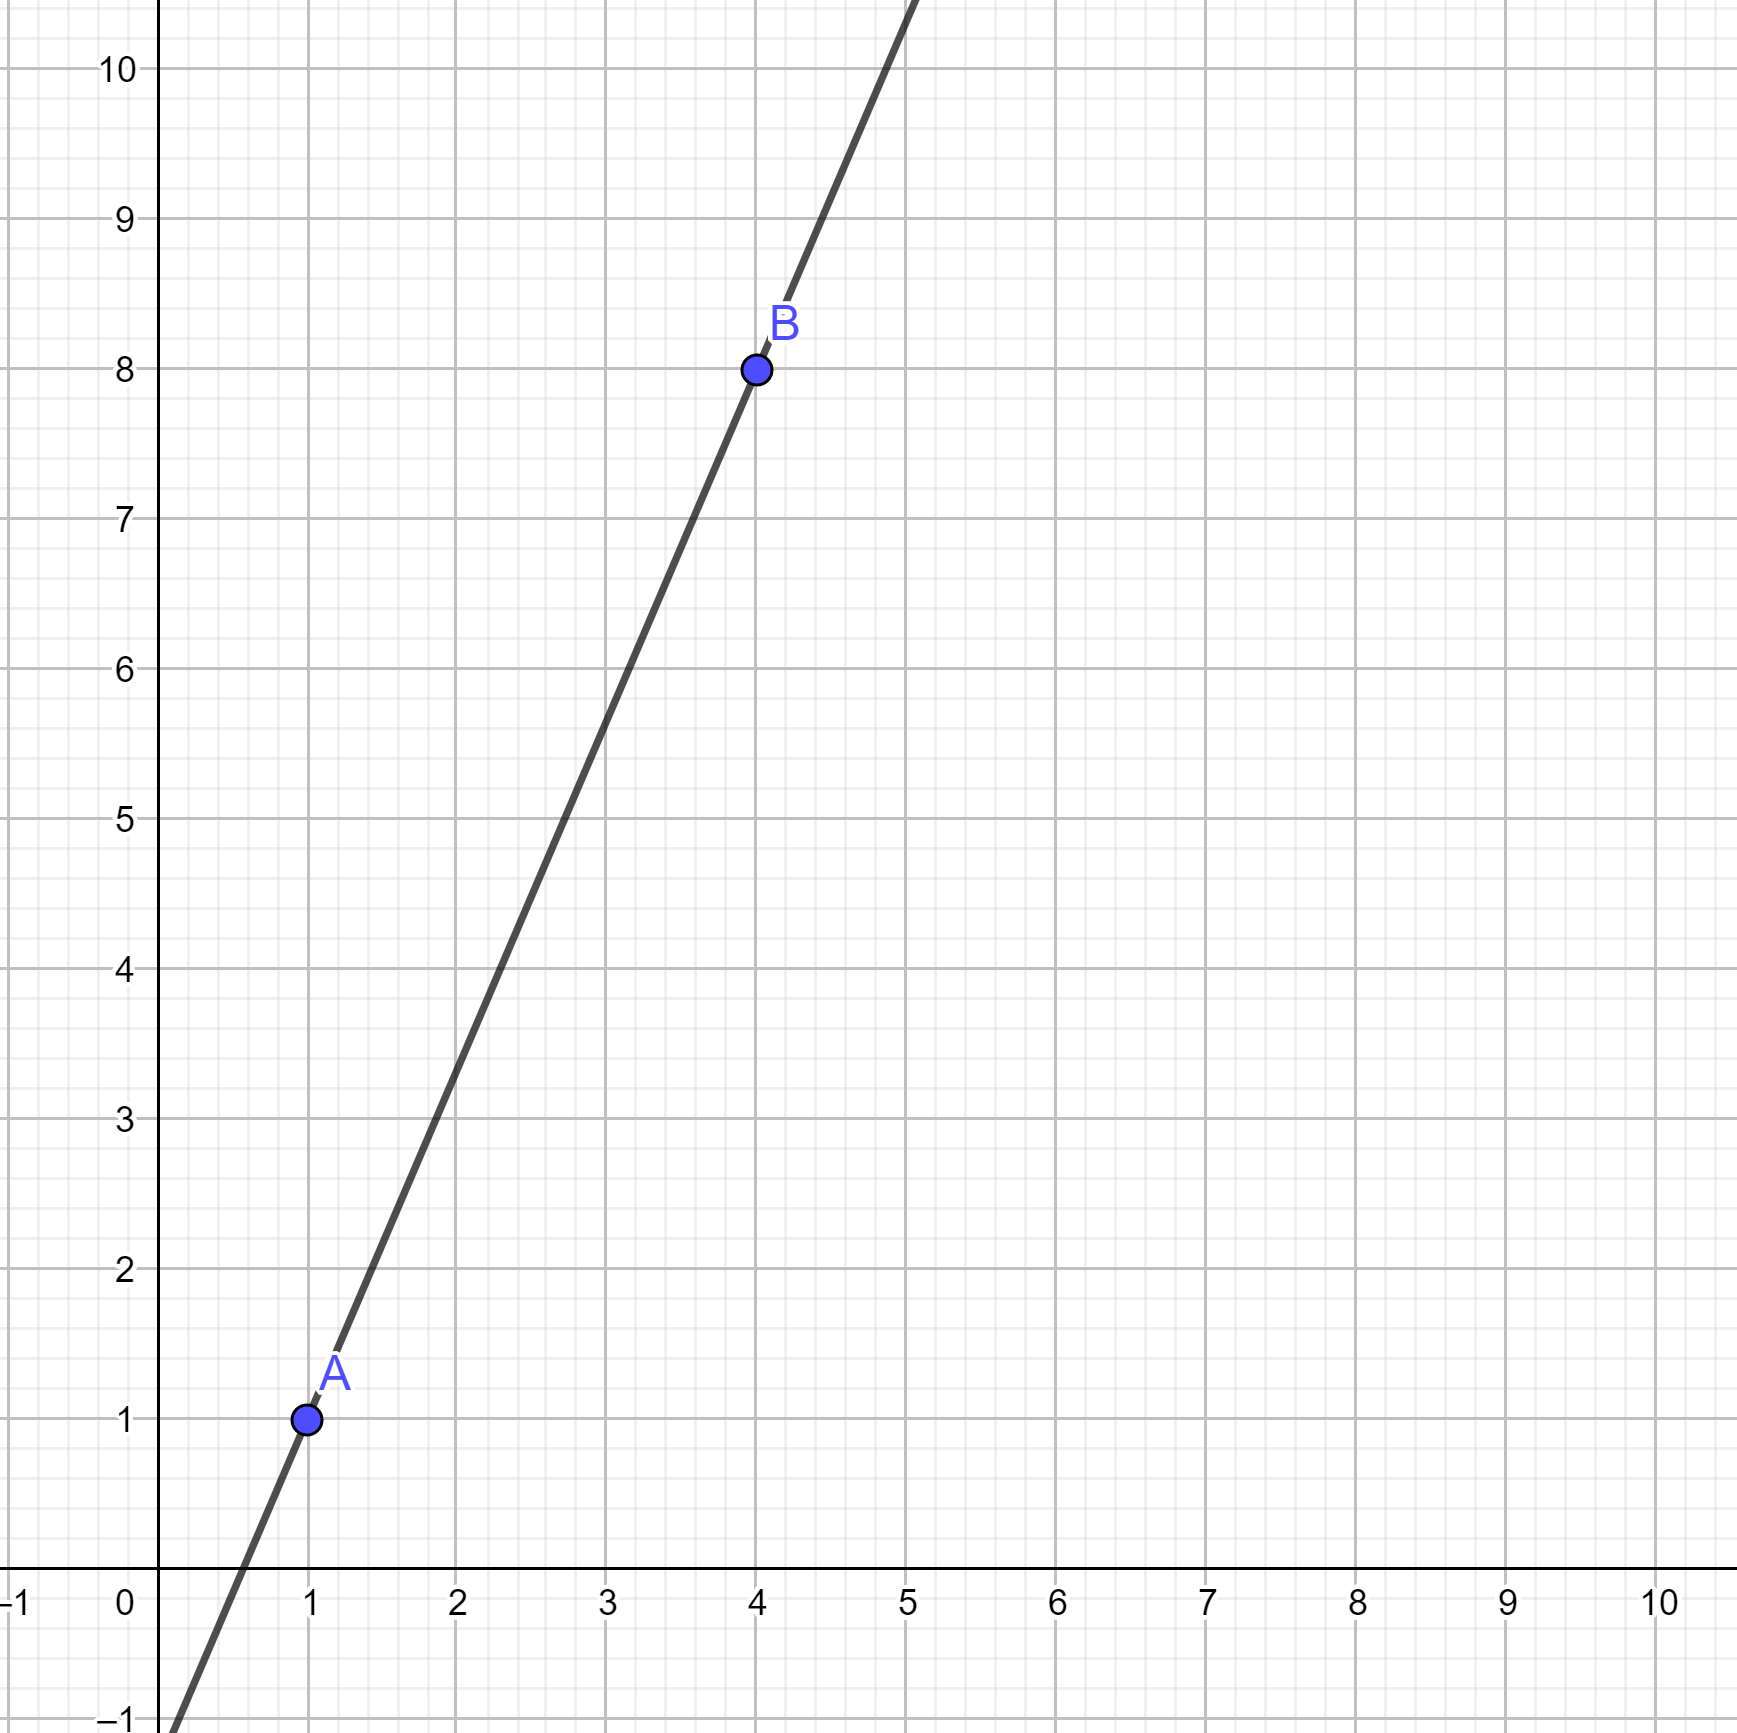
\includegraphics[scale=0.5]{img/droite2}		
	\end{center}

	\begin{multicols}{2}
		\begin{itemize}
		\item L'abscisse du point A est %+3;
		\item L'abscisse du point B est %+5;
		\item L'abscisse du point C est %-2;
		\item L'abscisse du point D est %-4.
		\item L'abscisse du point E est %\num{-5.5};
		\item L'abscisse du point O est %0;
	\end{itemize}
	\end{multicols}
\end{myex}


\begin{mydefs}
	\begin{itemize}
		\item Un repère orthogonal est formé par deux droites graduées perpendiculaires et de même origine. La droite horizontale est l'\hspace{6cm}, la verticale est l'%\kw{axe des ordonnées}.
		
		\item Un point du plan est repéré par deux nombres relatifs, ses %\kw{coordonnées}. 
		
		Le premier nombre est son \hspace{4cm}, le second son \hspace{4cm}. On note ces coordonnées $(abscisse \: ; \: ordonnée)$.
	\end{itemize}
\end{mydefs}


\begin{myexs}
	
		\begin{center}
			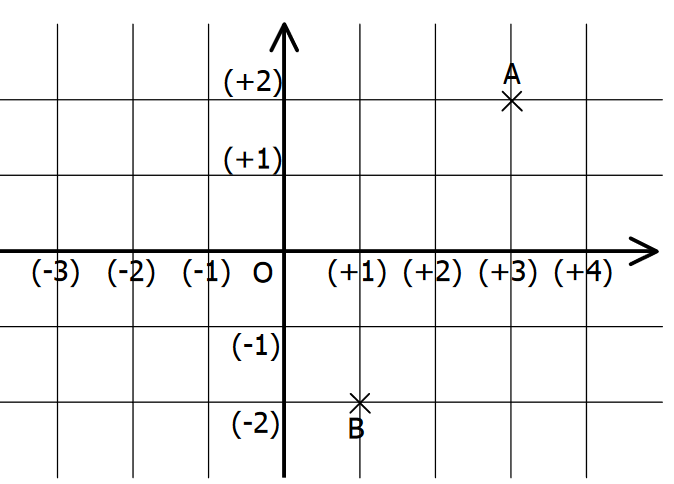
\includegraphics[scale=0.4]{repere}
		\end{center}
	

	\begin{itemize}
		\item L'abscisse du point $A$ est +3, son ordonnée est +2, ses coordonnées sont $(+3; +2)$.
		
		\item L'abscisse du point $B$ est +1, son ordonnée est -2, ses coordonnées sont $(+1; -2)$.
	\end{itemize}

\end{myexs}


\subsection{Comparaison}

\section{Addition et soustraction de deux nombres relatifs}


\begin{frame}
	\begin{myprop}
		Si deux nombres relatifs ont \kword{le même signe}, alors leur somme a :\pause
		\begin{itemize}
			\item \kword{le même signe};\pause
			\item pour distance à zéro, \pause \kword{la somme} de leurs distances à zéro.\pause
		\end{itemize}
	\end{myprop}


	\begin{myex}
		On veut calculer (+\num{2.4}) + (+\num{5.2}) : \pause
		
		Les deux nombres sont positifs :\pause
		\begin{itemize}
			\item leur somme est positive;\pause
			\item on ajoute les distances à zéro \\ $\num{2.4} + \num{5.2} = \num{7.6}$ \pause
			\item[$\Rightarrow$] (+\num{2.4}) + (+\num{5.2}) = \pause (+\num{7.6})
		\end{itemize}
	\end{myex}
\end{frame}


\begin{frame}
	\begin{myprop}
		Si deux nombres relatifs ont \kword{le même signe}, alors leur somme a :
		\begin{itemize}
			\item \kword{le même signe};
			\item pour distance à zéro,  \kword{la somme} de leurs distances à zéro. 
		\end{itemize}
	\end{myprop}
	
	
	\begin{myex}
		On veut calculer (-\num{4.6}) + (-\num{3.7}) :
		
		Les deux nombres sont négatifs :\pause
		\begin{itemize}
			\item leur somme est négative;\pause
			\item on ajoute les distances à zéro \\ $\num{4.6} + \num{3.7} = \num{8.3}$ \pause
			\item[$\Rightarrow$] (-\num{4.6}) + (-\num{3.7}) = \pause (-\num{8.3})
		\end{itemize}
	\end{myex}
\end{frame}


\begin{frame}
	\begin{myprop}
		Si deux nombres relatifs ont \kword{des signes différents}, alors leur somme a :\pause
		\begin{itemize}
			\item le signe du nombre qui à \kword{la plus grande distance à zéro}; \pause
			\item pour distance à zéro, \kword{la différence} de leurs distances à zéro. \pause
		\end{itemize}
	\end{myprop}


	\begin{myex}
		On veut calculer (-\num{2.4}) + (+\num{5.2}) : \pause
		
		Les deux nombres sont de signe différents : \pause
		\begin{itemize}
			\item (+ \num{5.2}) a la plus grande distance à zéro, \pause leur somme est positive; \pause
			\item on soustrait les distances à zéro  \pause \\ $\num{5.2} - \num{2.4} = \num{2.8}$ \pause
			\item[$\Rightarrow$] (-\num{2.4}) + (+\num{5.2}) = \pause (+\num{2.8})
		\end{itemize}
	\end{myex}
\end{frame}


\begin{frame}
	\begin{myprop}
		Si deux nombres relatifs ont \kword{des signes différents}, alors leur somme a :\pause
		\begin{itemize}
			\item le signe du nombre qui à \kword{la plus grande distance à zéro}; \pause
			\item pour distance à zéro, \kword{la différence} de leurs distances à zéro. \pause
		\end{itemize}
	\end{myprop}
	
	
	\begin{myex}
		On veut calculer (-\num{4.6}) + (+\num{3.7}) : \pause
		
		Les deux nombres sont de signe différents : \pause
		\begin{itemize}
			\item (- \num{4.6}) a la plus grande distance à zéro, leur somme est négative; \pause
			\item on soustrait les distances à zéro \pause \\ $\num{4.6} - \num{3.7} = \num{0.9}$ \pause
			\item[$\Rightarrow$] (-\num{4.6}) + (-\num{3.7}) = \pause (-\num{8.3})
		\end{itemize}
	\end{myex}
\end{frame}
\end{document}